\begin{figure}[t]
\centering
\subfigure[]{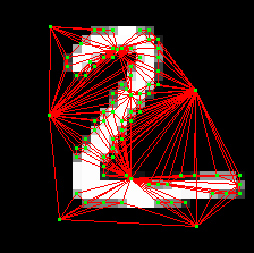
\includegraphics[scale=0.5]{bilder/knotenentferung_1}}
\subfigure[]{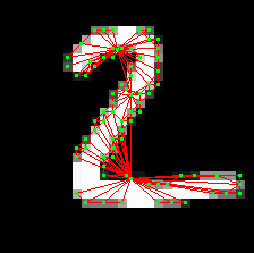
\includegraphics[scale=0.5]{bilder/knotenentferung_2}}
\caption[Entfernung irrelevanter Knoten]{Illustration der Entfernung irrelevanter Knoten eines Graphen, der über Quickshift eines Bildes aus dem \gls{MNIST} Datensatz gewonnen wurde.
(a) zeigt den Ursprungsgraphen der Segmentierung, wohingegen (b) die irrelevanten Knoten, die den Hintergrund beschreiben, entfernt.}
\label{fig:knotenentfernung}
\end{figure}
